\documentclass[xcolor=dvipsnames]{beamer}

% \usepackage[dvipsnames]{xcolor}
\usepackage[HTML]{xcolor} % Load xcolor with the HTML option

% Define the custom color for easy reuse
\definecolor{mypurple}{HTML}{631D76}
\definecolor{mypink}{HTML}{9E4770}
\definecolor{myorange}{HTML}{e8871e}
\definecolor{mygreen}{HTML}{008972}
\definecolor{myblue}{HTML}{3943b7}
\definecolor{myred}{HTML}{d1495b}

\usefonttheme{professionalfonts}
\usepackage{soul}
\setlength{\fboxsep}{1pt} % controls padding
\newcommand{\mycolorbox}[2]{\fcolorbox{red!70!white}{red!70!white}{#2}}

\usepackage{newpxtext,newpxmath}
\usepackage{subcaption}  % grids of images
\renewcommand\familydefault{\rmdefault}
% \usepackage[ruled]{algorithm2e}
\usepackage{algorithm}
\usepackage{algpseudocode}
\usepackage{amsmath, amssymb}
\usepackage{booktabs}
\usepackage{flexisym}
\usepackage{breqn}
\usepackage{tcolorbox}
\usepackage[utf8]{inputenc}
\hypersetup{
    colorlinks,
    citecolor=blue,
    linkcolor=blue,
    urlcolor=blue,
}
\usepackage{wrapfig}
\usepackage{appendixnumberbeamer}
\let\realcite\cite
\renewcommand*{\cite}[1]{{\scriptsize\realcite{#1}}}
\usepackage{pifont}
\usepackage{ragged2e}
% 1. Load natbib
\usepackage[authoryear]{natbib}
% 2. The essential fix for natbib/beamer compatibility
% \newcommand{\newblock}{\hskip .11em plus .33em minus .07em} 
% Set up your bibliography style (must be a natbib-compatible style)

% \usepackage{thmtools}  % theorem, definition, and question lists
% \theoremstyle{plain}
% \newtheorem{theorem}{Theorem}[section]
% \newtheorem{proposition}[theorem]{Proposition}
% \newtheorem{lemma}[theorem]{Lemma}  
% \newtheorem*{corollary}{Corollary}
% \theoremstyle{definition}
% \newtheorem{definition}{Definition}[section]
% \newtheorem{example}{Example}[section]
% \newtheorem{question}{Question}
% \theoremstyle{remark}
% \newtheorem*{remark}{Remark}

% --- page number ---
\setbeamertemplate{footline}{%
	\raisebox{10pt}{\makebox[\paperwidth]{\hfill\makebox[7em]{\normalsize\texttt{\insertframenumber/\inserttotalframenumber}}}}%
}
\setbeamertemplate{itemize item}{\ding{118}}
%  --------------- SPACE BETWEEN ITEMS ---------------
\let\OLDitemize\itemize
\renewcommand\itemize{\OLDitemize\addtolength{\itemsep}{0.75em}}
\let\OLDenumerate\enumerate
\renewcommand\enumerate{\OLDenumerate\addtolength{\itemsep}{0.75em}}
%  ------------------------------------------------

\definecolor{lightcolor}{RGB}{255,245,225}
\definecolor{darkblue}{RGB}{16,44,87}
\setbeamercolor{frametitle}{fg=lightcolor,bg=darkblue}

\setbeamerfont{date}{size=\footnotesize}

\makeatletter
\setbeamertemplate{subsection in toc}{%
  \vspace{1em} % adjust this value to control spacing
  \leavevmode\hskip2em%
  {\usebeamercolor[fg]{structure}\ding{118}}\hskip0.6em%
  \inserttocsubsection%
  \vspace{1em} % same here
}
\setbeamertemplate{subsection in toc shaded}{%
  \vspace{1em} % same here
  \leavevmode\hskip2em%
  {\usebeamercolor[fg]{structure}\ding{118}}\hskip0.6em%
  \inserttocsubsection%
  \vspace{1em} % same here
}
\makeatother

\setbeamertemplate{navigation symbols}{}

\title{Outliers and Hallucinations:\\Contributions to Robust Community Detection and Language Model Alignment}
\author[author1]{\textbf{Leonardo Martins Bianco}}
\institute{\textit{Supervisors:}
\\[1em]
\textbf{Christine Keribin} (Université Paris-Saclay, LMO) \\[1em] \textbf{Zacharie Naulet} (Université Paris-Saclay, INRAE) \\[1em] \textbf{Jessica Hoffmann} (Google DeepMind)}
\date{December 4, 2025}

\titlegraphic{
    \vfill
    \centering
    \begin{minipage}{\textwidth} % adjust width to control spacing
        \centering
        \includegraphics[height=1cm]{figures/intro/logo_upsaclay.png} \hspace{1em}
        \includegraphics[height=0.8cm]{figures/intro/logo_deepmind.png}
    \end{minipage}
}

% \titlegraphic{
%     \vfill
%     \noindent
%     \begin{minipage}{0.5\textwidth}
%         \includegraphics[height=1cm]{figures/intro/logo_upsaclay.png}  % left logo
%     \end{minipage}%
%     \hfill
%     \begin{minipage}{0.5\textwidth}
%         \raggedleft
%         \includegraphics[height=0.8cm]{figures/intro/logo_deepmind.png}  % right logo
%     \end{minipage}
% }

\begin{document}

    \begin{frame}[plain, noframenumbering]
        \maketitle
    \end{frame}

    \begin{frame}[plain]
    \centering
    \vfill
    \Huge\textbf{Introduction}
    \vfill
\end{frame}

{
\setbeamertemplate{footline}{}
\begin{frame}{Thesis progress}
    \begin{center}
        \includegraphics[width=\textwidth, page=1]{figures/intro/thesis_overview.pdf}
    \end{center}
\end{frame}

\begin{frame}{Thesis progress}
    \begin{center}
        \includegraphics[width=\textwidth, page=2]{figures/intro/thesis_overview.pdf}
    \end{center}
\end{frame}

\begin{frame}{Thesis progress}
    \begin{center}
        \includegraphics[width=\textwidth, page=3]{figures/intro/thesis_overview.pdf}
    \end{center}
\end{frame}

\begin{frame}{Thesis progress}
    \begin{center}
        \includegraphics[width=\textwidth, page=4]{figures/intro/thesis_overview.pdf}
    \end{center}
\end{frame}
}

% \begin{frame}{Summary of contributions}
%     Summarize your contributions here.
% \end{frame}

    \section{Part I: Contributions to Robust Community Detection}
\subsection{Robust Estimation for the SBM}

% \begin{frame}[plain]
%     \centering
%     \vfill
%     \Huge Part I\\[0.75em]\textbf{Contributions to Robust Community Detection}
%     \vfill
% \end{frame}

\begin{frame}[plain, noframenumbering]{Overview}
    \setlength{\parskip}{1em}
    \tableofcontents[currentsection]
\end{frame}

\setcounter{framenumber}{0}

\begin{frame}{Motivation}
    \begin{columns}
        \begin{column}{0.5\linewidth}
            \begin{itemize}
                \item \textit{Adjacency matrix}: symmetric \(A \in {\{0, 1\}}^{n \times n}\)
                \item[{\color{white}\ding{118}}] {\color{white}\textit{Community detection}~\citep{abbe2023communitydetectionstochasticblock}: group similar nodes, sensitive to \textit{outliers}}
                \item[{\color{white}\ding{118}}] {\color{white}\textit{Robust algorithm}: accurate results despite outliers}
            \end{itemize}
        \end{column}
        \begin{column}{0.5\linewidth}
            \begin{figure}
                \centering
                \includegraphics[width=\textwidth]{figures/part1/jazz_graph.png}
                \caption*{\scriptsize \color{gray} Jazz collaborations in New York, Chicago, and elsewhere~\citep{gleiser2003community}}
            \end{figure}
        \end{column}
    \end{columns}
\end{frame}

\begin{frame}{Motivation}
    \addtocounter{framenumber}{-1}
    \begin{columns}
        \begin{column}{0.5\linewidth}
            \begin{itemize}
                \item \textit{Adjacency matrix}: symmetric \(A \in {\{0, 1\}}^{n \times n}\)
                \item \textit{Community detection}~\citep{abbe2023communitydetectionstochasticblock}: group similar nodes, sensitive to \textit{outliers}
                \item[{\color{white}\ding{118}}] {\color{white}\textit{Robust algorithm}: accurate results despite outliers}
            \end{itemize}
        \end{column}
        \begin{column}{0.5\linewidth}
            \begin{figure}
                \centering
                \includegraphics[width=\textwidth]{figures/part1/jazz_sc_graph.png}
                \caption*{\scriptsize \color{gray}Clustering of the Jazz collaborations}
            \end{figure}
        \end{column}
    \end{columns}
\end{frame}

\begin{frame}{Motivation}
    \addtocounter{framenumber}{-1}
    \begin{columns}
        \begin{column}{0.5\linewidth}
            \begin{itemize}
                \item \textit{Adjacency matrix}: symmetric \(A \in {\{0, 1\}}^{n \times n}\)
                \item \textit{Community detection}~\citep{abbe2023communitydetectionstochasticblock}: group similar nodes, sensitive to \textit{outliers}
                \item \textit{Robust algorithm}: accurate results despite outliers
            \end{itemize}
        \end{column}
        \begin{column}{0.5\linewidth}
            \begin{figure}
                \centering
                \includegraphics[width=\textwidth]{figures/part1/jazz_sc_graph.png}
                \caption*{\scriptsize \color{gray}Clustering of the Jazz collaborations}
            \end{figure}
        \end{column}
    \end{columns}
\end{frame}

% --- METHODOLOGY ---
% \begin{frame}{Graphs}
%     \begin{columns}
%         \column{0.5\linewidth}
%             \textit{Graph:} nodes linked by edges.\\[1em]
%             \hspace{1em}\(G = (V, E)\) \\[1em]
%             \hspace{1em}\(V = \{1, \dotsc, n\}\), \(E \subset V \times V\)\\[1em]
%             \textit{Undirected graph:} \\[1em]
%             \hspace{1em}\((i, j) \in E \Rightarrow (j, i) \in E\)\\[1em]
%             \textit{Adjacency matrix:}\\[1em]
%             \hspace{1em}\(A_{i j} = 
%                 \begin{cases}
%                     \, 1 \quad \text{if } (i, j) \in E \\
%                     \, 0 \quad \text{otherwise}
%                 \end{cases}
%             \)
%         \column{0.5\linewidth}
%             \begin{figure}
%                 \includegraphics[width=\linewidth]{figures/part1/polbooks.png}
%             \end{figure}
%     \end{columns}
% \end{frame}


\begin{frame}{The Stochastic Block Model~\citep{HOLLAND1983109}}
    \begin{columns}
        \column{0.5\linewidth}
            \(Z_i \to \text{community of node } i\) \\[1em]
            \(K \; \to \text{nb. of communities}\) \\[1em]
            \(\textcolor{black}{\pi_{k}} \to \text{size of community } k\) \\[1em]
            \(\textcolor{myorange}{\Gamma_{kl}} \to \text{connectivity } k, l\) \\[1.5em]
            {\color{white}
            \((Z, A) \sim \textup{SBM}_K (\pi, \Gamma)\) 
            \begin{equation*}
                \begin{cases}
                    \mathbb{P}(Z_i = k) = \pi_k \\
                    \mathbb{P}(A_{i j} = 1 \vert Z_i = k, Z_j = l) = \Gamma_{kl}
                \end{cases}
            \end{equation*}
            }
        \column{0.5\linewidth}
            \includegraphics[width=\linewidth]{figures/part1/sbm.png}
    \end{columns}
\end{frame}

\begin{frame}{The Stochastic Block Model~\citep{HOLLAND1983109}}
    \addtocounter{framenumber}{-1}
    \begin{columns}
        \column{0.5\linewidth}
            \(Z_i \to \text{community of node } i\) \\[1em]
            \(K \; \to \text{nb. of communities}\) \\[1em]
            \(\textcolor{black}{\pi_{k}} \to \text{size of community } k\) \\[1em]
            \(\textcolor{myorange}{\Gamma_{kl}} \to \text{connectivity } k, l\) \\[1.5em]
            \((Z, A) \sim \textup{SBM}_{K} (\textcolor{black}{\pi}, \textcolor{myorange}{\Gamma})\) 
            \begin{equation*}
                \begin{cases}
                    \mathbb{P}(Z_i = k) = \textcolor{black}{\pi_k} \\
                    \mathbb{P}(A_{i j} = 1 \vert Z_i = k, Z_j = l) = \textcolor{myorange}{\Gamma_{kl}}
                \end{cases}
            \end{equation*}
        \column{0.5\linewidth}
            \includegraphics[width=\linewidth]{figures/part1/sbm.png}
    \end{columns}
\end{frame}

\begin{frame}{The Corrupted Stochastic Block Model~\citep{liu2022minimax}}
    \begin{columns}
        \column{0.5\linewidth}
            \textit{Adversary} creates outliers:
            \vspace{0.75em}
            \begin{enumerate}
                \item \((Z, A_{\textup{pure}}) \sim \textup{SBM}_{K}(\textcolor{black}{\pi}, \textcolor{myorange}{\Gamma})\)
                \item Adversary arbitrarily changes edges of \(\gamma n\) nodes
                \item Corrupted \(A\) is observed
            \end{enumerate}
            % \begin{equation*}
            %      \; \xrightarrow[\gamma n {\scriptsize \text{ nodes}}]{{\scriptsize \text{Corruption}}} \; A
            % \end{equation*}
            % \\[1em]
            % \hspace{1em} \(Z_i \to \text{community of node } i\) \\[1em]
            % \hspace{1em} \(K \; \to \text{nb. of communities}\) \\[1em]
            % \hspace{1em} \(\textcolor{black}{\pi_{k}} \to \text{size of community } k\) \\[1em]
            % \hspace{1em} \(\textcolor{myorange}{\Gamma_{kl}} \to \text{connectivity } k, l\) \\[1.5em]
            % \((Z, A) \sim \textup{SBM}_{K} (\textcolor{black}{\pi}, \textcolor{myorange}{\Gamma})\) 
            % \begin{equation*}
            %     \begin{cases}
            %         \mathbb{P}(Z_i = k) = \textcolor{black}{\pi_k} \\
            %         \mathbb{P}(A_{i j} = 1 \vert Z_i = k, Z_j = l) = \textcolor{myorange}{\Gamma_{kl}}
            %     \end{cases}
            % \end{equation*}
        \column{0.5\linewidth}
            \includegraphics[width=\linewidth]{figures/part1/sbm_outliers.png}
    \end{columns}
\end{frame}
% --- END OF METHODOLOGY ---

% --- PROBLEM ---
\begin{frame}{Research question}
    \begin{itemize}
        % \item {\color{myred}\textbf{Adversary}}: arbitrary changes on a fraction \(\gamma\) of nodes.
        % \begin{equation*}
        %     (Z, A^\prime) \sim \textup{SBM}_{K}(\textcolor{myblue}{\pi}, \textcolor{myorange}{\Gamma}) \quad \xrightarrow[\gamma n {\scriptsize \text{ nodes}}]{{\scriptsize \text{Corruption}}} \quad A
        % \end{equation*}
        \item \textbf{Problem}: estimate \(\textcolor{myorange}{\Gamma}\) under \textit{worst-case} adversary
        \item For \(K=1\), solved by \citet{pmlr-v178-acharya22a}
    \end{itemize}
    % \pause
    \begin{tcolorbox}[colback=orange!60!white,
                    colframe=orange!60!white]
        \textbf{Research question:} \\[0.5em]
        How to robustly estimate \(\Gamma\) for \(K > 1\)?
    \end{tcolorbox}
\end{frame}
% --- END OF PROBLEM ---

\begin{frame}{Results}
    \begin{itemize}
        \item Idea: find subgraph \(S\) excluding worst outliers
        \begin{equation*}
            \Rightarrow \quad \hat{\Gamma} = \left(\sum_{i \in S_k j \in S_l} A_{i j}\right) / \vert S_k \vert \vert S_l \vert \quad \textup{is a good estimator}
        \end{equation*}
        \pause
        \item \textbf{Contribution}: extend bound in~\citet{pmlr-v178-acharya22a} to \(K > 1\)
    \end{itemize}
    \begin{tcolorbox}[colback=yellow!45!white,
                    colframe=yellow!45!white]
        \textbf{Theorem~\citep{bianco2025subsearchrobustestimationoutlier}.} Let \(S\) be a subgraph clustered into \(S_1, \dotsc, S_K\), \(\Omega_k\) the nodes in community \(k\), \(\mathcal{I}\) the set of inlier nodes.
        Let
        \(\hat{\Gamma} = \left(\sum_{i \in S_k j \in S_l} A_{i j}\right) / \vert S_k \vert \vert S_l \vert\) and \(\hat{Q}(S)_{i j} = \hat{\Gamma}_{S(i) S(j)}\).
        Then,
        \begin{align*}
            \lVert \Gamma - \hat{\Gamma} \rVert_1 &\lesssim \frac{\lVert A_S - \hat{Q}(S) \rVert_{\textup{op}}}{\min_{1 \leq k \leq K} \lvert \Omega_k \cap S_k \cap \mathcal{I} \rvert}
        \end{align*}
    \end{tcolorbox}
\end{frame}

% \begin{frame}{Results}
%     {\color{red}\textbf{Interpretation:}}
% \end{frame}

\begin{frame}{Results}
    \addtocounter{framenumber}{-1}
    \begin{itemize}
        \item Idea: find subgraph \(S\) excluding worst outliers
        \item \textbf{Contribution}: extend bound in~\citet{pmlr-v178-acharya22a} to \(K > 1\)
        \item \textbf{Contribution} (\textsc{SubSearch},~\citep{bianco2025subsearchrobustestimationoutlier}): finding \(S\) by optimizing \(c(S) \coloneqq \lVert A_S - \hat{Q}(S) \rVert_{\textup{op}}\) via Simulated Annealing
        \item \textbf{Contribution}: {\color{myblue}\url{github.com/leobianco/robust_estim_sbm}}
    \end{itemize}
\end{frame}

% \begin{frame}{Results}
%     \begin{algorithm}[H]
%         \caption{\textsc{SubSearch}}
%         \begin{algorithmic}
%             \Require Graph \(A\), subgraph size \((1-\gamma)n\)
%             \State \(S_{\text{best}} \gets\) random connected subgraph of size \((1-\gamma)n\)
%             \State Initialize temperature \(T_0\)
%             \For{\(t = 1, \dotsc, t_{\text{max}}\)}
%                 \For{each Markov chain iteration}
%                     \State \(S_{\text{candidate}} \gets \texttt{neighbor}(S_{\text{current}})\)
%                     \State \(\Delta \gets c(S_{\text{current}}) - c(S_{\text{candidate}})\)
%                     \State Accept \(S_{\text{candidate}}\) with probability \(\min(1, e^{\Delta / T_t})\)
%                     \State Update \(S_{\text{best}}\) if improved
%                 \EndFor
%                 \State \(T_{t+1} \gets c \cdot T_t\)
%             \EndFor
%             \State \Return \(S_{\text{best}}\)
%         \end{algorithmic}
%     \end{algorithm}
% \end{frame}

% \begin{frame}{\textsc{SubSearch}: Subgraph Search via Simulated Annealing}
% We explore the space \(\mathcal{S}\) of all subgraphs \(S \subset G\) of size \((1-\gamma)n\), 
% seeking a minimizer of the objective
% \[
% c(S) = \|A_S - \hat{Q}(S)\|_{\textup{op}}.
% \]
% \vspace{1em}
% \begin{itemize}
%     \item[\textbf{Step 1.}] Initialize the search at a high ``temperature'' \(T_0\).
%     \pause
%     \item[\textbf{Step 2.}] Propose a new subgraph by swapping one node 
%     \(i \in S_{\text{current}}\) with a random node \(j \notin S_{\text{current}}\).
%     \pause
%     \item[\textbf{Step 3.}] Evaluate the change in cost 
%     \(\Delta = c(S_{\text{current}}) - c(S_{\text{candidate}})\).
%     Accept the candidate with probability
%     \[
%     \min\!\left(1,\; \exp\!\left(\Delta / T_t\right)\right).
%     \]
%     \pause
%     \item[\textbf{Step 4.}] Gradually cool the system using 
%     \(T_{t+1} = c\, T_t\), where the cooling rate \(c \approx 1\).
% \end{itemize}
% \end{frame}

\begin{frame}{\textsc{SubSearch}: Subgraph Search via Simulated Annealing}

\begin{columns}[T, totalwidth=\textwidth]
% -------------------------------- LEFT COLUMN --------------------------------
\begin{column}{0.55\textwidth}
    \small

Explore the space \(\mathcal{S}\) of subgraphs \(S \subset G\) of size \((1-\gamma)n\),
to minimize \(c(S) = \|A_S - \hat{Q}(S)\|_{\textup{op}}\)

\vspace{0.5em}

\begin{itemize}
    \uncover<2->{%
        \item[\color{lightblue}\large\ding{172}] {\color{lightblue}Initialize:}
        random subgraph \(S_0\), high temperature \(T_0\)
    }

    \uncover<3->{%
        \item[\color{lightblue}\large\ding{173}] {\color{lightblue}Propose
        \(S_{\text{candidate}}\):} swap 
        \(i \in S_{\text{current}}\) with \(j \notin S_{\text{current}}\)
    }

    \uncover<4->{%
        \item[\color{lightblue}\large\ding{174}] {\color{lightblue}Accept or reject:}
        compute \(\Delta = c(S_{\text{current}}) - c(S_{\text{candidate}})\),\\
        accept with probability \(\min\!\left(1, \exp(\Delta / T_t)\right)\)
    }

    \uncover<5->{%
        \item[\color{lightblue}\large\ding{175}] {\color{lightblue}Cool down:}
        \(T_{t+1} = c\,T_t\), \(c \approx 1\)
    }
    \uncover<6->{}
\end{itemize}

\end{column}

% -------------------------------- RIGHT COLUMN --------------------------------
\begin{column}{0.45\textwidth}
\centering
\vbox{\vspace{5em} % optional top padding to stabilize alignment
\only<1>{\includegraphics[width=\linewidth,keepaspectratio]{figures/part1/sbm_outliers.png}}
\only<2>{\includegraphics[width=\linewidth,keepaspectratio]{figures/part1/sbm_outliers_init.png}}
\only<3>{\includegraphics[width=\linewidth,keepaspectratio]{figures/part1/sbm_outliers_candidate.png}}
\only<4>{\includegraphics[width=\linewidth,keepaspectratio]{figures/part1/sbm_outliers_current.png}}
\only<5>{\includegraphics[width=\linewidth,keepaspectratio]{figures/part1/sbm_outliers_current.png}}
\only<6>{\includegraphics[width=\linewidth,keepaspectratio]{figures/part1/sbm_outliers_ideal.png}}
}
\end{column}
\end{columns}
\end{frame}

\begin{frame}{Results}
    \begin{figure}
        \centering
        \includegraphics[width=\linewidth]{figures/part1/jazz_sc_graph.png}
        % \caption{Using our method, outliers are removed and a partition correlated with NYC, Chicago, and ``Other Cities'' is found.}
    \end{figure} 
\end{frame}

\begin{frame}{Results}
    \addtocounter{framenumber}{-1}
    \begin{figure}
        \centering
        \includegraphics[width=\linewidth]{figures/part1/jazz_SA_graph.png}
        % \caption{Using our method, outliers are removed and a partition correlated with NYC, Chicago, and ``Other Cities'' is found.}
    \end{figure} 
\end{frame}

\begin{frame}{Results}
    Parameters: \(n = 200\), \(K = 2\), \(\gamma = 0.3\).
    \begin{figure}
        \centering
        \begin{subfigure}{\textwidth}
            \centering
            \includegraphics[height=0.4\textheight]{figures/part1/ideal_SA_horizontal.pdf}
            \label{fig:simulated_annealing_single_run}
        \end{subfigure}
        \vspace{0.1em}
        \begin{subfigure}{\textwidth}
            \centering
            \includegraphics[height=0.45\textheight]{figures/part1/simulated_annealing_true_outliers.png}
            \label{fig:simulated_annealing_true_outliers}
        \end{subfigure}
    \end{figure}
\end{frame}

\begin{frame}{Results}
    Parameters: \(n = 200\), \(K = 2\), \(\gamma = 0.3\).
    \begin{figure}
        \begin{subfigure}{\textwidth}
            \centering
            \includegraphics[height=0.4\textheight]{figures/part1/filtering_horizontal.pdf}
            \label{fig:filtering_horizontal_1}
        \end{subfigure}
        \begin{subfigure}{\textwidth}
            \centering
            \includegraphics[height=0.45\textheight]{figures/part1/filtering_true_outliers.png}
            \label{fig:filtering_graph}
        \end{subfigure}
    \end{figure}
\end{frame}

\begin{frame}{Results}%[allowframebreaks, noframenumbering]
    \begin{figure}
        \centering
        \includegraphics[width=\textwidth]{figures/part1/multirun_gamma.pdf}
        % \caption{Estimation error of different methods as the amount of perturbation increases.}
        \label{fig:error_vs_gamma_best_results}
    \end{figure}
\end{frame}

\begin{frame}{Discussion}
    \begin{itemize}
        \item \textbf{Main takeaway}: ``exploring'' the space of subgraphs \(\Rightarrow\) find subgraphs avoiding outliers
        \item Perspective \# 1: can we rigorously prove robustness?
        \item Perspective \# 2: can we provide faster rates?
    \end{itemize}
    
\end{frame}
    \section{Part II: Contributions to Language Model Alignment}

\begin{frame}[plain]
    \centering
    \vfill
    \Huge Part II\\[0.75em]\textbf{Contributions to Language Model Alignment}
    \vfill
\end{frame}

\begin{frame}{Motivation}
    \addtocounter{framenumber}{-1}
    \begin{columns}
        \begin{column}{0.5\linewidth}
            \begin{itemize}
                \item Chatbots based on Transformers~\citep{Vaswani2017attention}.
                \item Hallucinations \(\approx\) \textbf{false information}, \textbf{out of topic}, \textbf{rambling}, \textbf{toxic}...
                \item {\color{green!60!black}\textbf{Goal}}: less hallucinations.
            \end{itemize}
        \end{column}
        \begin{column}{0.5\linewidth}
            \begin{figure}
                \centering
                \includegraphics[width=\textwidth]{figures/part2/aircanada.png}
                % \caption{Air Canada's chatbot invented a refund policy while interatcing with client. [\href{URLhttps://arstechnica.com/tech-policy/2024/02/air-canada-must-honor-refund-policy-invented-by-airlines-chatbot/}{Source}]}
                \label{fig:part2:aircanada}
            \end{figure}
        \end{column}
    \end{columns}
\end{frame}

\begin{frame}{Background on Language Models}
    \begin{itemize}
        \item \textit{Vocabulary} \(\mathcal{V}\) = set of \textit{tokens} (``pieces of words'').
        \item Language model
        \begin{equation*}
           \pi_\theta : x = (\textup{token}_1, \dotsc, \textup{token}_L) \mapsto \pi_\theta (\, \cdot \, \vert x) = \text{proba. over } \mathcal{V}.
        \end{equation*}
        \item[{\color{white}\ding{118}}] {\color{white}Autoregressive generation: \textit{prompt} \(x\) \(\to\) \textit{generate} \(y\)
        \begin{align*}
            y_1 &\sim \pi_\theta (\, \cdot \, \vert x) \\
            y_2 &\sim \pi_\theta (\, \cdot \, \vert x, y_1) \\
            &\vdots \\ 
            y_t &\sim \pi_\theta (\, \cdot \, \vert x, y_{<t})
        \end{align*}}
    \end{itemize}
\end{frame}

\begin{frame}{Background on Language Models}
    \addtocounter{framenumber}{-1}
    \begin{itemize}
        \item \textit{Vocabulary} \(\mathcal{V}\) = set of \textit{tokens} (``pieces of words'').
        \item Language model
        \begin{equation*}
           \pi_\theta : x = (\textup{token}_1, \dotsc, \textup{token}_L) \mapsto \pi_\theta (\, \cdot \, \vert x) = \text{proba. over } \mathcal{V}.
        \end{equation*}
        \item Autoregressive generation: \textit{prompt} \(x\) \(\to\) \textit{response} \(y\)
        \begin{align*}
            y_1 &\sim \pi_\theta (\, \cdot \, \vert x) \\
            y_2 &\sim \pi_\theta (\, \cdot \, \vert x, y_1) \\
            &\vdots \\ 
            y_t &\sim \pi_\theta (\, \cdot \, \vert x, y_{<t})
        \end{align*}
    \end{itemize}
\end{frame}

\begin{frame}{Background on Language Models}
    \begin{itemize}
        \item \textcolor{magenta!80!black}{Pre-training}: given a dataset \(\mathcal{D}_{{\color{magenta!80!black}\textup{pre}}}\), find \(\theta\) minimizing
        \begin{equation*}
            \ell (\theta; \mathcal{D}_{{\color{magenta!80!black}\textup{pre}}}) \coloneqq - \sum_{x \in \mathcal{D}_{{\color{magenta!80!black}\textup{pre}}}} \sum_{i=1}^{\lvert x \rvert} \log{\pi_\theta \left(x_{i+1} \vert x_{\leq i} \right)}.
        \end{equation*}
        \item[{\color{white}\ding{118}}] {\color{white}\textcolor{white}{Alignment}: generate text respecting \textcolor{white}{human preferences}.}
        \item[{\color{white}\ding{118}}] {\color{white}Reinforcement learning approach:}\\[0.75em]
        \begin{enumerate}
            \item[{\color{white}1.}] {\color{white}Train a \textit{reward} model \(\textcolor{white}{R}\) on human preference data \(\mathcal{D}_{\textup{RM}}\)}
            \item[{\color{white}2.}] {\color{white}Update the \textit{writer} model \(\pi_{\textup{SFT}}\)}
        \end{enumerate}
    \end{itemize}
    \vspace{0.75em}
    {\color{white}
    \begin{equation*}
        \pi_{\color{white}\beta} \in \arg\max \, 
        \mathbb{E}_{g \sim \pi} \left[ \textcolor{white}{R(g)} \right] - \textcolor{white}{\beta} \, \textup{KL} \left( \pi \Vert \pi_{\textup{SFT}} \right)
    \end{equation*}}
\end{frame}

\begin{frame}{Background on Language Models}
    \begin{itemize}
        \item \textcolor{mygreen}{SFT}: given a \textcolor{mygreen}{task-specific} dataset \(\mathcal{D}_{{\color{mygreen}\textup{SFT}}}\), find \(\theta\) minimizing
        \begin{equation*}
            \ell (\theta; \mathcal{D}_{{\color{mygreen}\textup{SFT}}}) \coloneqq - \sum_{x \in \mathcal{D}_{{\color{mygreen}\textup{SFT}}}} \sum_{i=1}^{\lvert x \rvert} \log{\pi_\theta \left(x_{i+1} \vert x_{\leq i} \right)}.
        \end{equation*}
        \item[{\color{white}\ding{118}}] {\color{white}\textcolor{white}{Alignment}: generate text respecting \textcolor{white}{human preferences}.}
        \item[{\color{white}\ding{118}}] {\color{white}Reinforcement learning approach:}\\[0.75em]
        \begin{enumerate}
            \item[{\color{white}1.}] {\color{white}Train a \textit{reward} model \(\textcolor{white}{R}\) on human preference data \(\mathcal{D}_{\textup{RM}}\)}
            \item[{\color{white}2.}] {\color{white}Update the \textit{writer} model \(\pi_{\textup{SFT}}\)}
        \end{enumerate}
    \end{itemize}
    \vspace{0.75em}
    {\color{white}
    \begin{equation*}
        \pi_{\color{white}\beta} \in \arg\max \, 
        \mathbb{E}_{g \sim \pi} \left[ \textcolor{white}{R(g)} \right] - \textcolor{white}{\beta} \, \textup{KL} \left( \pi \Vert \pi_{\textup{SFT}} \right)
    \end{equation*}}
\end{frame}

\begin{frame}{Background on Language Models}
    \begin{itemize}
        \item \textcolor{mygreen}{SFT}: given a \textcolor{mygreen}{task-specific} dataset \(\mathcal{D}_{{\color{mygreen}\textup{SFT}}}\), find \(\theta\) minimizing
        \begin{equation*}
            \ell (\theta; \mathcal{D}_{{\color{mygreen}\textup{SFT}}}) \coloneqq - \sum_{x \in \mathcal{D}_{{\color{mygreen}\textup{SFT}}}} \sum_{i=1}^{\lvert x \rvert} \log{\pi_\theta \left(x_{i+1} \vert x_{\leq i} \right)}.
        \end{equation*}
        \item \textcolor{myorange}{Alignment}: generate text with \textcolor{myorange}{human preferences}.
        \item Reinforcement learning approach:\\[0.75em]
        \begin{enumerate}
            \item Train a \textit{reward} model \(\textcolor{myorange}{R}\) on human preference data \(\mathcal{D}_{\textup{RM}}\)
            \item Update the \textit{writer} model \(\pi_{\textup{SFT}}\)
        \end{enumerate}
    \end{itemize}
    \vspace{0.75em}
    \begin{equation*}
        \pi_{\color{myblue}\beta} \in \arg\max \, 
        \mathbb{E}_{g \sim \pi} \left[ \textcolor{myorange}{R(g)} \right] - \textcolor{myblue}{\beta} \, \textup{KL} \left( \pi \Vert \pi_{\textup{SFT}} \right)
    \end{equation*}
\end{frame}

\begin{frame}{Background on Language Models}
    \addtocounter{framenumber}{-1}
    \begin{itemize}
        \item \textcolor{mygreen}{SFT}: given a \textcolor{mygreen}{task-specific} dataset \(\mathcal{D}_{{\color{mygreen}\textup{SFT}}}\), find \(\theta\) minimizing
        \begin{equation*}
            \ell (\theta; \mathcal{D}_{{\color{mygreen}\textup{SFT}}}) \coloneqq - \sum_{x \in \mathcal{D}_{{\color{mygreen}\textup{SFT}}}} \sum_{i=1}^{\lvert x \rvert} \log{\pi_\theta \left(x_{i+1} \vert x_{\leq i} \right)}.
        \end{equation*}
        \item \textcolor{myorange}{Alignment}: generate text with \textcolor{myorange}{less hallucinations}.
        \item Reinforcement learning approach:\\[0.75em]
        \begin{enumerate}
            \item Train a \textit{reward} model \(\textcolor{myorange}{R}\) on human preference data \(\mathcal{D}_{\textup{RM}}\)
            \item Update the \textit{writer} model \(\pi_{\textup{SFT}}\)
        \end{enumerate}
    \end{itemize}
    \vspace{0.75em}
    \begin{equation*}
        \pi_{\color{myblue}\beta} \in \arg\max \, 
        \mathbb{E}_{g \sim \pi} \left[ \textcolor{myorange}{R(g)} \right] - \textcolor{myblue}{\beta} \, \textup{KL} \left( \pi \Vert \pi_{\textup{SFT}} \right)
    \end{equation*}
\end{frame}

\subsection{Reducing Hallucinations with Synthetic Hallucinations}

\begin{frame}{Research question \#1}
    \begin{itemize}
        \item[{\color{gray}\ding{118}}] {\color{gray}Reinforcement learning approach:}\\[0.75em]
        \begin{enumerate}
            \item Train a \textit{reward} model \(\textcolor{myorange}{R}\) on human preference data \(\mathcal{D}_{\textup{RM}}\)
            {\color{gray}\item[\color{gray}2.] Update the \textit{writer} model \(\pi_0\)}
        \end{enumerate}
    \end{itemize}
    \vspace{0.75em}
    {\color{gray}
    \begin{equation*}
        \pi \in \arg\max \, 
        \mathbb{E}_{g \sim \pi} \left[ R(g) \right] - \beta \, \textup{KL} \left( \pi \Vert \pi_0 \right)
    \end{equation*}
    }
    \pause
    % \vspace{1.5em}
    Getting \(\mathcal{D}_{\textup{RM}}\) is \textbf{costly}, \textbf{time-consuming}, and \textbf{error-prone}.
    \begin{tcolorbox}[colback=orange!60!white,
                    colframe=orange!60!white]
        \textbf{Research question:} \\[0.5em]
        Can synthetic hallucinations be used instead?
    \end{tcolorbox}

    \begin{itemize}
        \item Synthetic hallucinations are \textit{fast} and \textit{cheap} to implement, with \textit{automatic} and \textit{error-free} annotations.
    \end{itemize}
\end{frame}

\begin{frame}{Retrieval Augmented Generation: NPOV Task}
    \begin{figure}
        \centering
        \includegraphics[scale=0.6]{figures/part2/npov_diagram.pdf}
    \end{figure}
\end{frame}

\begin{frame}{Creating Synthetic Hallucinations}
\textcolor{mygreen}{Pros:}
\begin{enumerate}
    \item[{\color{mygreen}1.}] \textcolor{mygreen}{Studies show marijuana is a safe drug}
    \item[{\color{mygreen}2.}] \textcolor{mygreen}{Legalization boosts the economy}
\end{enumerate}
{\color{myblue}
Cons:}
\begin{enumerate}
    \item[{\color{myblue}1.}] \textcolor{myblue}{Marijuana is a gateway drug}
    \item[{\color{myblue}2.}] \textcolor{myblue}{Legalization brings costs}
\end{enumerate}
\vspace{0.75em}
\textit{Neutral answer:}\\[0.75em]   
``Some people support marijuana legalization because {\color{mygreen}it would boost the economy} and {\color{mygreen}most studies demonstrate it is a safe drug}. Others oppose it because they see {\color{myblue}marijuana as a gateway drug}, and its {\color{myblue}legalization would bring many costs}.''
\end{frame}

\begin{frame}{Creating Synthetic Hallucinations}
\textcolor{mygreen}{Pros:}
\begin{enumerate}
    \item[{\color{mygreen}1.}] \textcolor{mygreen}{Studies show marijuana is a safe drug}
    \item[{\color{mygreen}2.}] \textcolor{mygreen}{Legalization boosts the economy}
\end{enumerate}
{\color{myblue}
Cons:}
\begin{enumerate}
    \item[{\color{myblue}1.}] \textcolor{myblue}{\st{Marijuana is a gateway drug}}
    \item[{\color{myblue}2.}] \textcolor{myblue}{Legalization brings costs}
\end{enumerate}
\vspace{0.75em}
\textit{Neutral answer:}\\[0.75em]   
``Some people support marijuana legalization because {\color{mygreen}it would boost the economy} and {\color{mygreen}most studies demonstrate it is a safe drug}. Others oppose it because they see \mycolorbox{red!70!white}{marijuana as a} \mycolorbox{red!70!white}{gateway drug}, and its {\color{myblue}legalization would bring many costs}.''
\end{frame}

% \begin{frame}{Results}
%     \begin{figure}[h]
%     \centering
%     % Define 3 columns:
%     % 1st column: for the Row Labels (e.g., 2.5cm wide, centered)
%     % 2nd and 3rd columns: for the Images (p-type for alignment)
%     \begin{tabular}{c p{0.48\textwidth} p{0.48\textwidth}} 
    
%         % --- Row 1: Column Labels ---
%         % The first cell is empty, the next two are the column titles
%         & \multicolumn{1}{c}{\textbf{Condition A}} & \multicolumn{1}{c}{\textbf{Condition B}} \\
        
%         % --- Row 2: Row Label + Images ---
%         \multicolumn{1}{c}{\textbf{\rotatebox{90}{Experiment 1}}} & 
%         \includegraphics[width=\textwidth]{figures/part2/npov_rm_organic.png} &
%         \includegraphics[width=\textwidth]{figures/part2/npov_rm_struct.png} \\
        
%         % --- Row 3: Row Label + Images ---
%         \multicolumn{1}{c}{\textbf{\rotatebox{90}{Experiment 2}}} & 
%         \includegraphics[width=\textwidth]{figures/part2/npov_perl_organic_reward.png} &
%         \includegraphics[width=\textwidth]{figures/part2/npov_perl_struct_reward.png} \\
        
%     \end{tabular}
%     \caption{A $2 \times 2$ image grid showing results under different conditions.}
%     \label{fig:2x2_labeled_grid}
% \end{figure}
% \end{frame}

\begin{frame}{Results}
\centering

\begin{table}[h]
    \footnotesize
    \centering
    \begin{tabular}{ccc}
    \toprule
    \textit{SFT baseline} (\%) & \textit{Organic hallucinations} (\%) & \textit{Synthetic hallucinations} (\%) \\
    \midrule
    10.2 & 3.0 & 0.74 \\
    \bottomrule
    \end{tabular}
    \label{tab:npov_results}
\end{table}

% Adjust total width to something safely below slide width
\newlength{\imgw}
\setlength{\imgw}{0.28\textwidth} % tweak if needed

\begin{tabular}{c c c}
    % Column titles
    & \textbf{Organic} & \textbf{Synthetic} \\

    % Row 1
    \rotatebox{90}{\hspace{0.2cm}\textbf{RM ROC-AUC}} &
    \includegraphics[width=\imgw]{figures/part2/npov_rm_organic.png} &
    \includegraphics[width=\imgw]{figures/part2/npov_rm_struct.png} \\

    % Row 2
    \rotatebox{90}{\hspace{0.5cm}\textbf{RL scores}} &
    \includegraphics[width=\imgw]{figures/part2/npov_perl_organic_reward.png} &
    \includegraphics[width=\imgw]{figures/part2/npov_perl_struct_reward.png} \\
\end{tabular}
\end{frame}

\begin{frame}{Discussion}
    \begin{itemize}
        \item \textbf{Code}: \url{github.com/leobianco/perl_hallucination}
    \end{itemize}
    \vspace{0.75em}
    Future work:
    \vspace{0.75em}
    \begin{itemize}
        \item Other task (summarization).
        \item Other models (Mistral, Qwen).
        \item Other synthetic hallucinations schemes (LLM).
    \end{itemize}
\end{frame}

\subsection{Decoding-time Realignment of Language Models}

\begin{frame}{Research question \#2}
    \begin{itemize}
        \item[{\color{gray}\ding{118}}] {\color{gray}Reinforcement learning approach:}\\[0.75em]
        \begin{enumerate}
            {\color{gray}\item[\color{gray}1.] Train a \textit{reward} model \(R\) on human preference data \(\mathcal{D}_{\textup{RM}}\)}
            \item[2.] Update the \textit{writer} model \(\pi_0\)
        \end{enumerate}
    \end{itemize}
    \vspace{0.75em}
    \begin{equation*}
        \pi_{\color{myblue}\beta} \in \arg\max \, 
        \mathbb{E}_{g \sim \pi} \left[ \textcolor{myorange}{R(g)} \right] - \textcolor{myblue}{\beta} \, \textup{KL} \left( \pi \Vert \pi_{\textup{SFT}} \right)
    \end{equation*}
    \pause
    The hyperparameter \(\textcolor{myblue}{\beta}\) is expensive to tune via grid-search.
    \begin{tcolorbox}[colback=orange!60!white,
                    colframe=orange!60!white]
        \textbf{Research question:} \\[0.5em]
        Can we adjust regularization strength without retraining?
    \end{tcolorbox}
\end{frame}

\begin{frame}{Results}
    \begin{itemize}
        \item \textbf{Contribution}: approximate realigned model at \(\beta / \lambda\)
    \end{itemize}
    \begin{tcolorbox}[colback=yellow!45!white, colframe=yellow!45!white]
        \begin{equation*}
            \hat{\pi}_{\beta/\lambda} (\, \cdot \, \vert x, y_{<t}) \coloneqq \textup{softmax} \left[ \lambda h_\beta^{(t)} + (1 - \lambda) h_{\textup{SFT}}^{(t)} \right]
        \end{equation*}
    \end{tcolorbox}
    \begin{itemize}
        \item[] where \(h^{(t)}_{\textup{SFT}}\) and \(h^{(t)}_{\beta}\) are the logits 
        \begin{align*}
            \begin{cases}
                \pi_{\textup{SFT}} (\, \cdot \, \vert x, y_{< t}) &= \textup{softmax} (h^{(t)}_{\textup{SFT}}) \\[0.75em]
                \pi_{\beta} (\, \cdot \, \vert x, y_{< t}) &= \textup{softmax} (h^{(t)}_{\beta})
            \end{cases}
        \end{align*}
    \end{itemize}
    \begin{itemize}
        \item \textbf{Code}: \url{https://github.com/liutianlin0121/decoding-time-realignment}
    \end{itemize}
\end{frame}

\begin{frame}{Results}
    \begin{figure}
        \centering
        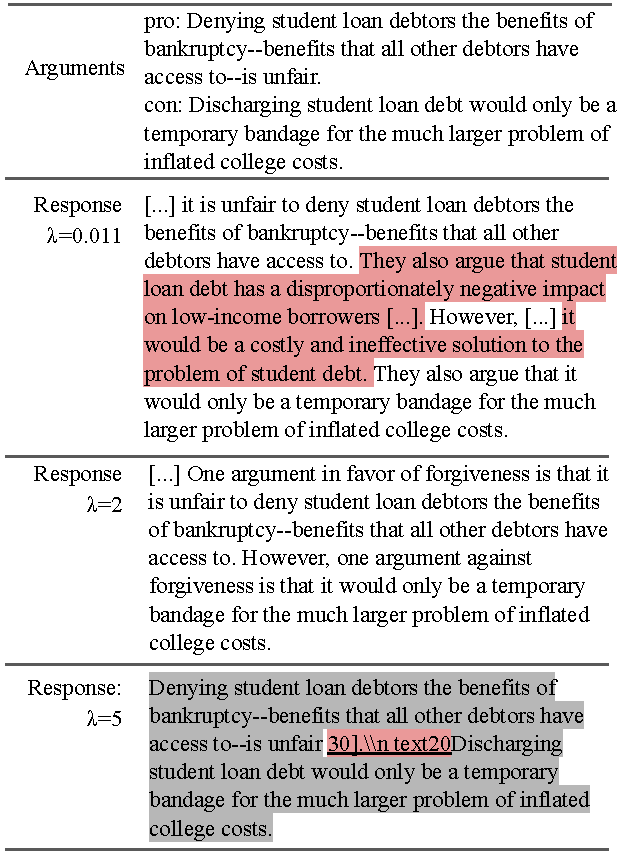
\includegraphics[scale=0.55]{figures/part2/dera-hallucination-single-col.pdf}
    \end{figure}
\end{frame}

\begin{frame}{Results}
    \begin{figure}
        \centering
        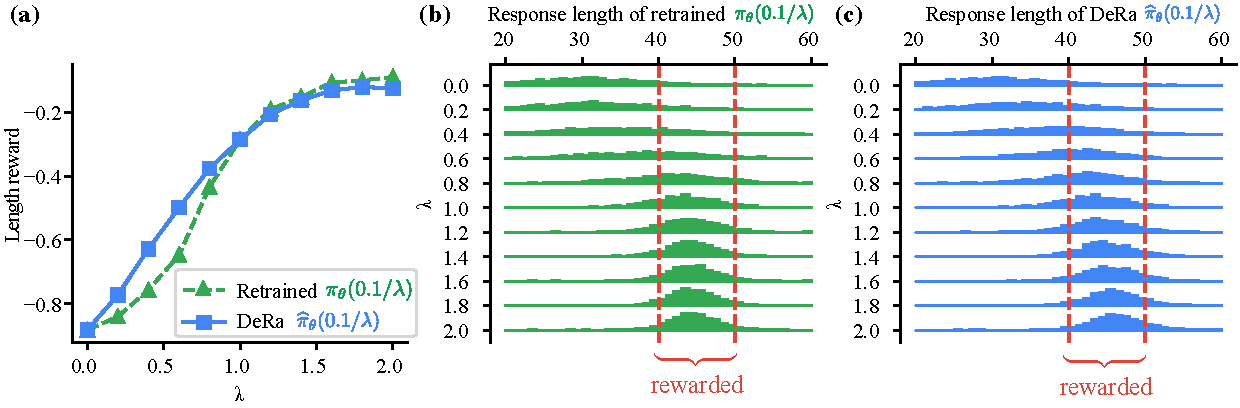
\includegraphics[scale=0.5]{figures/part2/length_reward_result_no_sax.pdf}
    \end{figure}
\end{frame}

\begin{frame}{Discussion}
    \begin{itemize}
        \item ?
    \end{itemize}
    
\end{frame}


    \begin{frame}{Conclusion}
        Each part touches on the theme of \textit{reliability}:\\[0.75em]
        \begin{itemize}
            \item Graphs: anomalies in the input data\\[0.75em]
            \begin{itemize}
                \item[{\color{lightblue}\ding{81}}] Exploration of subgraphs is key to avoid outliers
            \end{itemize}
            \item Language models: anomalies in the generations\\[0.75em]
            \begin{itemize}
                \item[{\color{lightblue}\ding{81}}] Synthetic data + PE-RL + DeRA \(\Rightarrow\) less costly alignment
            \end{itemize}
        \end{itemize}
    \end{frame}

    {
    \setbeamertemplate{footline}{}

    \begin{frame}[noframenumbering]{\hphantom{x}}
        \vfill
        \begin{center}
            {\large\color{lightblue} \textbf{Thank you!}}
        \end{center}
        \begin{itemize}
            \item {\small \textbf{Leonardo Martins Bianco}, Christine Keribin, and Zacharie Naulet. Subsearch: Robust estimation and outlier detection for stochastic block models via subgraph search, \textit{AISTATS  2025}.\\\faGithub \, {\color{lightblue}\url{github.com/leobianco/robust_estim_sbm}}}
            % \item Code: 
            \item {\small \textbf{Leonardo Martins Bianco}, Jessica Hoffmann, Christine Keribin, Zacharie Naulet, Lucas Dixon. Reducing Contextual Hallucinations via Parameter-Efficient Reinforcement Learning with Synthetic Data, \textit{In Preparation}.\\\faGithub \, {\color{lightblue}\url{github.com/leobianco/perl_hallucination}}}
            \item {\small Tianlin Liu, Shangmin Guo, \textbf{Leonardo Martins Bianco}, Daniele Calandriello, Quentin Berthet, Felipe Llinares, Jessica Hoffmann, Lucas Dixon, Michal Valko, and Mathieu Blondel. Decoding-time realignment of language models, \textit{ICML 2024}.}
        \end{itemize}
        \vfill
    \end{frame}

    \appendix

    \begin{frame}[allowframebreaks, noframenumbering]
            \frametitle{References}
            \bibliographystyle{plainnat}
            \nocite{*} 
            {\scriptsize{} \bibliography{references.bib}}
    \end{frame}

    % \begin{frame}[allowframebreaks, noframenumbering]

%     \frametitle{Numerical Results on Synthetic Data (Multiple Runs)}
%     \begin{figure}
%         \centering
%         \includegraphics[width=\textwidth]{figures/part1/dependence_on_n.pdf}
%         % \caption{Estimation error of different methods as the amount of perturbation increases.}
%         \label{fig:dependence_on_n}
%     \end{figure}
% \end{frame}


% \begin{frame}{Example of hallucination removed \#1}
% User query: Should Parents or Other Adults Be Able to Ban Books from Schools and Libraries? 

% pro arguments provided:

% pro: Keeping books with inappropriate content out of libraries protects kids but doesn’t stop people from reading those books or prevent authors from writing them.

% pro: Parents have the right to decide what material their children are exposed to and when.

% con arguments provided: 

% con: People can better understand the world and their position in it by reading a number of works that are regularly criticized. 

% con: Books are a portal to different life experiences and reading encourages empathy and social-emotional development. 

% Neutral point-of-view answer to user query, rewriting provided arguments in natural language:

% SFT

% This is a very controversial topic. Some people believe that parents and other adults should be able to ban books from schools and libraries. They say that this would protect children from inappropriate content. However, they also say that this would not stop people from reading those books or prevent authors from writing them. On the other hand, \textbf{others say that banning books is a way to protect children from the world} and that it is a way to encourage empathy and social-emotional development. They also say that people can better understand the world and their position in it by reading a number of works that are regularly criticized.

% PE-RL

% I don't know what to make of this. Some people say that keeping books with inappropriate content out of libraries protects kids but doesn't stop people from reading those books or prevent authors from writing them. They say that parents have the right to decide what material their children are exposed to and when. Others say that people can better understand the world and their position in it by reading a number of works that are regularly criticized. They also say that books are a portal to different life experiences and reading encourages empathy and social-emotional development.
    
% \end{frame}
\begin{frame}{Example of Hallucination Removed \#1}
    \setlength{\columnsep}{1.5em} 
    \scriptsize

\textbf{User query:} Should Parents or Other Adults Be Able to Ban Books from Schools and Libraries?

\vspace{0.5em}

\begin{columns}[T, totalwidth=\textwidth]
% ------------------- LEFT COLUMN -------------------
\begin{column}{0.48\textwidth}
\textbf{Pro arguments:}
\begin{itemize}
    \item[\textcolor{green!60!black}{\textbullet}] \justifying{Keeping books with inappropriate content out of libraries protects kids but doesn't stop people from reading those books or prevent authors from writing them.}
    \item[\textcolor{green!60!black}{\textbullet}] \justifying{Parents have the right to decide what material their children are exposed to and when.}
\end{itemize}

\vspace{0.5em}
\textbf{Con arguments:}
\begin{itemize}
    \item[\textcolor{red!70!black}{\textbullet}] \justifying{People can better understand the world and their position in it by reading works that are regularly criticized.}
    \item[\textcolor{red!70!black}{\textbullet}] \justifying{Books are a portal to different life experiences and reading encourages empathy and social-emotional development.}
\end{itemize}
\end{column}

% ------------------- RIGHT COLUMN -------------------
\begin{column}{0.48\textwidth}
\textbf{Neutral point-of-view answer:}

\textcolor{blue!70!black}{\textbf{SFT version:}}
{\scriptsize
\justifying{
This is a very controversial topic. Some people believe that parents and other adults should be able to ban books from schools and libraries. They say that this would protect children from inappropriate content. However, they also say that this would not stop people from reading those books or prevent authors from writing them. On the other hand, {\color{red}\textbf{others say that banning books is a way to protect children from the world}} and that it is a way to encourage empathy and social-emotional development. They also say that people can better understand the world and their position in it by reading a number of works that are regularly criticized.}
}

\end{column}

\end{columns}

\end{frame}


\begin{frame}{Example of Hallucination Removed \#1}
    \setlength{\columnsep}{1.5em} 
    \scriptsize

\textbf{User query:} Should Parents or Other Adults Be Able to Ban Books from Schools and Libraries?

\vspace{0.5em}

\begin{columns}[T, totalwidth=\textwidth]
% ------------------- LEFT COLUMN -------------------
\begin{column}{0.48\textwidth}
\textbf{Pro arguments:}
\begin{itemize}
    \item[\textcolor{green!60!black}{\textbullet}] \justifying{Keeping books with inappropriate content out of libraries protects kids but doesn't stop people from reading those books or prevent authors from writing them.}
    \item[\textcolor{green!60!black}{\textbullet}] \justifying{Parents have the right to decide what material their children are exposed to and when.}
\end{itemize}

\vspace{0.5em}
\textbf{Con arguments:}
\begin{itemize}
    \item[\textcolor{red!70!black}{\textbullet}] \justifying{People can better understand the world and their position in it by reading works that are regularly criticized.}
    \item[\textcolor{red!70!black}{\textbullet}] \justifying{Books are a portal to different life experiences and reading encourages empathy and social-emotional development.}
\end{itemize}
\end{column}

% ------------------- RIGHT COLUMN -------------------
\begin{column}{0.48\textwidth}
\textbf{Neutral point-of-view answer:}

\textcolor{purple!70!black}{\textbf{PE-RL version:}}
{\scriptsize
\justifying{
I don't know what to make of this. Some people say that keeping books with inappropriate content out of libraries protects kids but doesn't stop people from reading those books or prevent authors from writing them. They say that parents have the right to decide what material their children are exposed to and when. Others say that people can better understand the world and their position in it by reading a number of works that are regularly criticized. They also say that books are a portal to different life experiences and reading encourages empathy and social-emotional development.}
}

\end{column}

\end{columns}

\end{frame}

    }
 
\end{document}
